\chapter{Background and Related Work}

In this chapter, we will start with the introductions of most important theoretical concepts and frameworks to establish a foundation for the subsequent discussion of global illumination approaches. Then we will make a short survey on various approaches and their strenghts and weakness when dealing with different phenomena. Afterwards we will hightlight GPU-based techniques applied on Monte Carlo ray tracing and photon mapping and discuss some open issues of the current approach for the introduction of our new approach in the following chapter. 


%%%%%%%%%%%%%%%%%%%%%%%%%%%%%%%%%%%%%%%%%%%%%%%%%%%%%%%%%%%%%%%%%%%%%%%%%%

\section{Radiometry Introduction}
Radiometry is the basic terminology to describe light which is crucial to simulation. First of all, some basic quantities have to be introduced, the related symbols are going to be defined here as well for further use.

\subsection{Important Quantities} 

\begin{table}[ht]
\begin{center}
	
	\renewcommand{\arraystretch}{1.2}
	\begin{tabular}{ | l | l | l |}     	
	\hline 

	Symbol & Quantity & Unit \\
	\cline{1-3}

	% \(Q_{\lambda}\) 	& 		Spectral radiant energy 		& 		\(J nm^{-1} \) \\
	\(Q\) 			& 		Radiant Energy 				& 		\(j\) \\ 
	\(\Phi\) 			& 		Radiant flux 					& 		\(W\) \\ 
	\(I\) 			& 		Radiant intensity 				& 		\(W sr^{-1}\) \\
	\(E\)			&		Irradiance (incident) 			&		\(W m^{-2}\) \\  
	\(L\)			&		Radiance						&		\(W m^{-2} sr^{-1}\) \\ 
	
	\hline

	\end{tabular}
\end{center} 
\caption{Important Radiometry Quantities}
\label{tab:radiometry_quantities}
\end{table}

\emph{Radiant energy}, \(Q\), is the energy of a collection of photons which is the basic quantity in lighting. 

\emph{Radiant flux} , \(\Phi\), is the time rate of the flow of radiant energy passing through a surface or region of space. Total emission from a light source is generally described in terms of flux. \ref{fig:flux_point_light} shows the flux emitted from a point light source measured by the total amount of energy passing through an virtual sphere around the light. 

\begin{figure}[htp] 
    \centering 
    \fbox{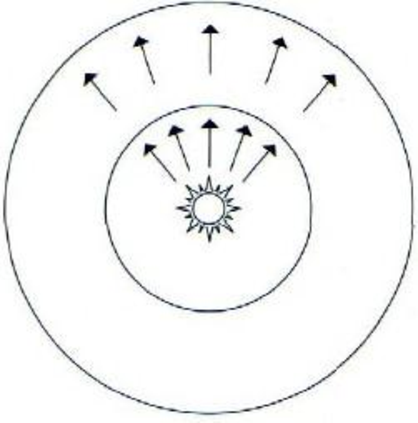
\includegraphics{imgs/flux.pdf}}
    \renewcommand{\thefigure}{\thechapter.\arabic{figure}}
    \caption[]{Radiant flux from a point light source is passing through the spheres around the light.}
    \label{fig:flux_point_light} 
\end{figure} 

\emph{Irradiance}, \(E\), is the incident (arriving at a surface location) \emph{radiant flux area density}, which is defined as the differential flux per differential area. While \emph{Radiant exitance} denoted by \(M\) is area density of flux leaving a surface.  

\begin{equation}
E(x) = \frac{d\Phi}{dA}
\end{equation}

\emph{Radiance}, \(L\), is the radiant flux per unit solid angle per unit projected area: 

\begin{equation}
L(x, \overrightarrow{\omega}) = \frac{d^{2}\Phi}{\cos{\theta} \cdot dA \cdot d\overrightarrow{\omega}}
\end{equation}

Where \(x\) is the position and \(\overrightarrow{\omega}\) is the direction. 

Radiance is the most important quantity in rendering simulation since it closely represent the color. Also radiance can be considered as the number of photons arriving per time at a small area from a given direction. Radiant energy can be computed by integrating the radiance field over all directions \(\Omega\) and area \(A\).

\begin{equation} 
\Phi = \int_{A}\int_{\Omega}L(x, \overrightarrow{\omega})(\overrightarrow{\omega} \cdot \overrightarrow{n})d\overrightarrow{\omega}dx
\label{eq:flux_from_radiance}
\end{equation} 

\begin{figure}[htp] 
    \centering 
    \fbox{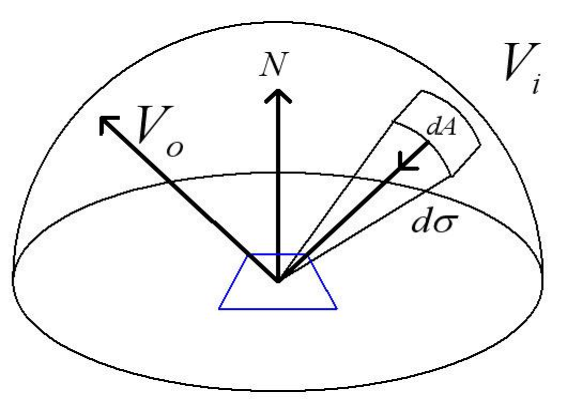
\includegraphics{imgs/solid_angle_sphere.pdf}}
    \renewcommand{\thefigure}{\thechapter.\arabic{figure}}
    \caption[]{Radiance, L, is defined as the radiant flux per unit solid angle, \(\overrightarrow{\omega}\), per unit projected area, \(dA\)}
    \label{fig:solid_angle_sphere} 
\end{figure}

The solid angle used in equation \ref{eq:flux_from_radiance} can be thought as representation of both a direction and an infinitesimal area. Therefore solid angle can also be expressed in spherical coordinates (\(\theta, \phi\))

\begin{figure}[htp] 
    \centering 
    \fbox{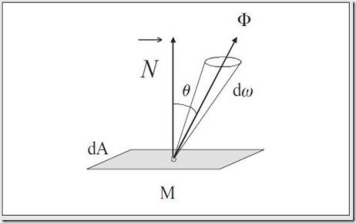
\includegraphics{imgs/radiance_solid_angle.pdf}}
    \renewcommand{\thefigure}{\thechapter.\arabic{figure}}
    \caption[]{Radiance, L, is defined as the radiant flux per unit solid angle, \(\overrightarrow{\omega}\), per unit projected area, \(dA\)}
    \label{fig:radiance_solid_angle} 
\end{figure} 

%%%%%%%%%%%%%%%%%%%%%%%%%%%%%%%%%%%%%%%%%%%%%%%%%%%%%%%%%%%%%%%%%%%%%%%%%%

\section{Fundamentals of Global Illumination}
With the basic knowledge of radiometry, we will introduced a theoretical framework as the basis of global illumination. There are several components are included in this framework, light source, reflectance and visibilty. We will look at these components firstly and then get to the rendering equation describing the interaction between light and an surface with no participating media. 

\subsection{Light Source} 
As the light in the form of photons is emitted from light sources initially, the lighting becomes an essential input of the model. There are several types of light sources widely used in Computer Graphics such as point, directional and area lights. The radiance of lighting emitted from light sources is denoted as \( L_{e} \). 

We can measure the intensity of light source in \emph{wattage}. Take a point light source for example, the power this light can emit is denoted by \(\Phi\), the emitted light distribute uniformly in all directions, the irradiance, \(E\), can be computed at a surface as: 

\begin{equation}
E(x) = \frac{\Phi \cos{\theta}}{4\pi r^{2}} 
\end{equation}

Where \(r\) is the distance from \(x\) to the light source and \(\theta\) is the angle between the surface normal and the direction to the light source. From the equation we can intuitively tell a surface facing the source will receive more photons per area than a surface that is oriented differently.   

\subsection{Reflectance} 
\begin{figure}[htp] 
    \centering 
    \fbox{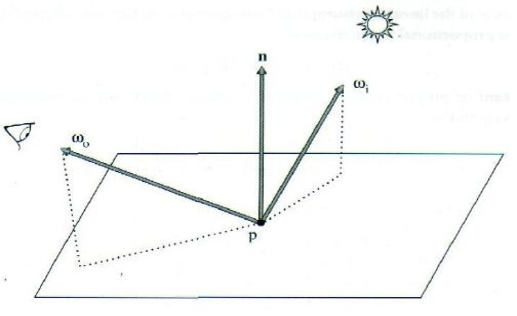
\includegraphics{imgs/brdf.pdf}}
    \renewcommand{\thefigure}{\thechapter.\arabic{figure}}
    \caption[]{The geometric setup of BRDF. }
    \label{fig:brdf} 
\end{figure} 

The \emph{Bidirectional Reflectance Distribution Function}, BRDF, is the mathematic tool describing the reflectiona of light encounters an surface. To define the BRDF, the geometric configuration is shown in figure \ref{fig:brdf}. \(\omega_{i}\) is the incident lighting direction, \(\omega_{o}\) is the direction in which the reflected light leaving from the surface, \(n\) is the normal vector at the location \(p\) on the surface. Given the incident radiance \(L_{i}(p, \omega_{i})\), we are finding out the outgoing radiance to the viewer, \(L_{o}(p, \omega_{o})\). 

The BRDF, \(f_{r}\), defines the relationship between differential reflected radiance and differential irradiance: 

\begin{equation}
f_{r} = \frac{dL_{o}(p, \omega_{o})}{dE(p, \omega_{i})} = \frac{dL_{o}(p, \omega_{o})}{L_{i}(p, \omega_{i})(\omega_{i} \cdot n)d\omega{i}}
\label{eq:brdf} 
\end{equation} 

There are two important properties of BRDF used in rendering. The first one is the Helmholtz's law of reciprocity, that is given any pair of directions \( (\omega_{i}, \omega_{o} ) \), we have: 

\begin{equation}
f_{r}(p, \omega_{i}, \omega_{o}) = f_r(p, \omega_{o}, \omega_{i})
\end{equation}

Another important physical property of BRDF is energy conservation, stating that the total reflected energy is less than or equal to the incident energy. For all direction \( \omega_{o} \).

\begin{equation}
 \int_{\Omega}f_{r}(p, \omega_{i}, \omega_{o})L_{i}(p, \omega_{i})(\omega_{i} \cdot n)d\omega_{i} \leq 1 , \forall \omega_{i}
\end{equation}

Note that there are special cases exists in the BRDF model, one is the \emph{Lambertian} BRDF in which the outgoding direction  is independent from the incident direction. Another extreme case is the perfect mirror reflection BRDF which is a Dirac delta function making the incident direction \(\omega_{i}\) mirrored at the surface normal at the \(p\) on the surfacee. BRDFs including thesee two special case is often broadly classified as directional diffuse, glossy and specular. 

Given the definition of BRDF, we can introduce the basic render equation, also known as \emph{local illumination model} by integrating the equation \ref{eq:brdf} over the sphere of incident directions around location \(p\), the left side of the equation will be the outgoding radiance in direction \(\omega_{o}\). 

\begin{equation}
L_{o}(p, \omega_{o}) = \int_{\Omega}f_{r}(p, \omega_{i}, \omega_{o})L_{i}(p, \omega_{i})(\omega_{i} \cdot n)d\omega_{i}
\label{eq:local_render_equation}
\end{equation}

Where \(\Omega\) is the hemisphere of incoming directions at \(p\).

\subsection{Visibility} 
Another important component is the visibility computation. It is often modeled as a binary function denoted by \(V(x, x')\). 
We have following equation: 

  \begin{equation}
    V(x, x')=\left\{
    \begin{array}{ll}
      1  & \text{x and x' are mutually visible} \\
      0  & \text{otherwise}
    \end{array}
    \right.
  \end{equation}

Ray casting is the mose widely used operator to determine the closest surface in a direction by shooting a ray into the scene trying to find the closest intersection point with the surface. We will discuss ray casting and ray tracing technique further in section \ref{subsec:classic_rt}.

Another more complicated model of visibility is non-binary function occures between surface point a area light source, this model is used to simulate the soft shadows.  \cite{Hasenfratz2003} is a full survey of existing shadow methods dedicated to real-time rendering of soft shadows. 

\subsection{Light Transport Equation} 

The local rendering equation used to describe the direct lighting effect is too simple for simulating real-world lighting effect, indirect lighting has to be introduced to this model as well. Therefore we introduce the Light Transport Equation (LTE) in this section to form the mathematical basis for all global illumination algorithms. The LTE is also known as Rendering Equation(RE) which is introduced in the first time in \cite{Kajiya:1986:RE:15922.15902}. We use LTE term here to be distinguished from the local rendering equation, also it is more suitable with context of global illumination. The LTE states that the outgoing radiance \(L_{o}\) at location \(p\) on the surface in the direction \(\omega_{o}\) is the sum of emitted radiance \(L_{e}\) and reflected radiance \(L_{r}\). The reflected radiance can be computed using the local rendering equation \ref{eq:local_render_equation} so we have final LTE shown in equation \ref{eq:lte}. 

\begin{equation}
L_{o}(p, \omega_{o}) = L_{e}(p, \omega_{o}) + \int_{\Omega}f_{r}(p, \omega_{i}, \omega_{o})L_{i}(p, \omega_{i})(\omega_{i} \cdot n)d\omega_{i}
\label{eq:lte}
\end{equation}  

%%%%%%%%%%%%%%%%%%%%%%%%%%%%%%%%%%%%%%%%%%%%%%%%%%%%%%%%%%%%%%%%%%%%%%%%%%

\section{Related Work}
In this section, we will review the several the most popular approaches to compute the global illuminations including radiosity , Monte Carlo ray tracing and photon mapping and previous work related to these approaches. 


\subsection{Radiosity}

Radiosity, also known as finite element approach, is a classic solution to solving the LTE. It was introduced by  \citeauthor{Goral:1984:MIL:964965.808601} in \citep{Goral:1984:MIL:964965.808601} and became an active field that was drawing quite research interest. The underlying idea is to tessellate the surfaces into finite small sub-surfaces called patches as geometric primitives and solve the LTE with them. Solving LTE using radiosity requires several input. First of all the radiosity value for diffuse surfaces or the BRDF for the non-diffuse surfaces need to be stored for all the patches in the scene. Then it requires a known linear system of equations called form factors which denote the amount of light transport between two patches. 

Computing the form factors is the most time consuming part because of the initial time compxity of \(O(n^{2})\) of linking \(n\) patches, however when this precomputing is done the entire scene can be rendered very efficiently. Therefore a lot researchers were focusing on minimizing this performance hit. \citeauthor{Hanrahan:1991:RHR:127719.122740}\cite{Hanrahan:1991:RHR:127719.122740} introduced a technique that constructs a hierarchical representation of the form factor matrix to reduce the computation. \citeauthor{Holzschuch94anefficient}\cite{Holzschuch94anefficient} followed the hierarchical structure and introduced a progressive refinement strategy resulting the form factor only is computed when needed to evaluate the energy transfers from a given surface. 


\subsection{Monte Carlo Ray Tracing} 
\label{sec:mc_rt} 

\begin{figure}[htp] 
\begin{center}
    \fbox{
	\subfigure[Test subfigure 1]{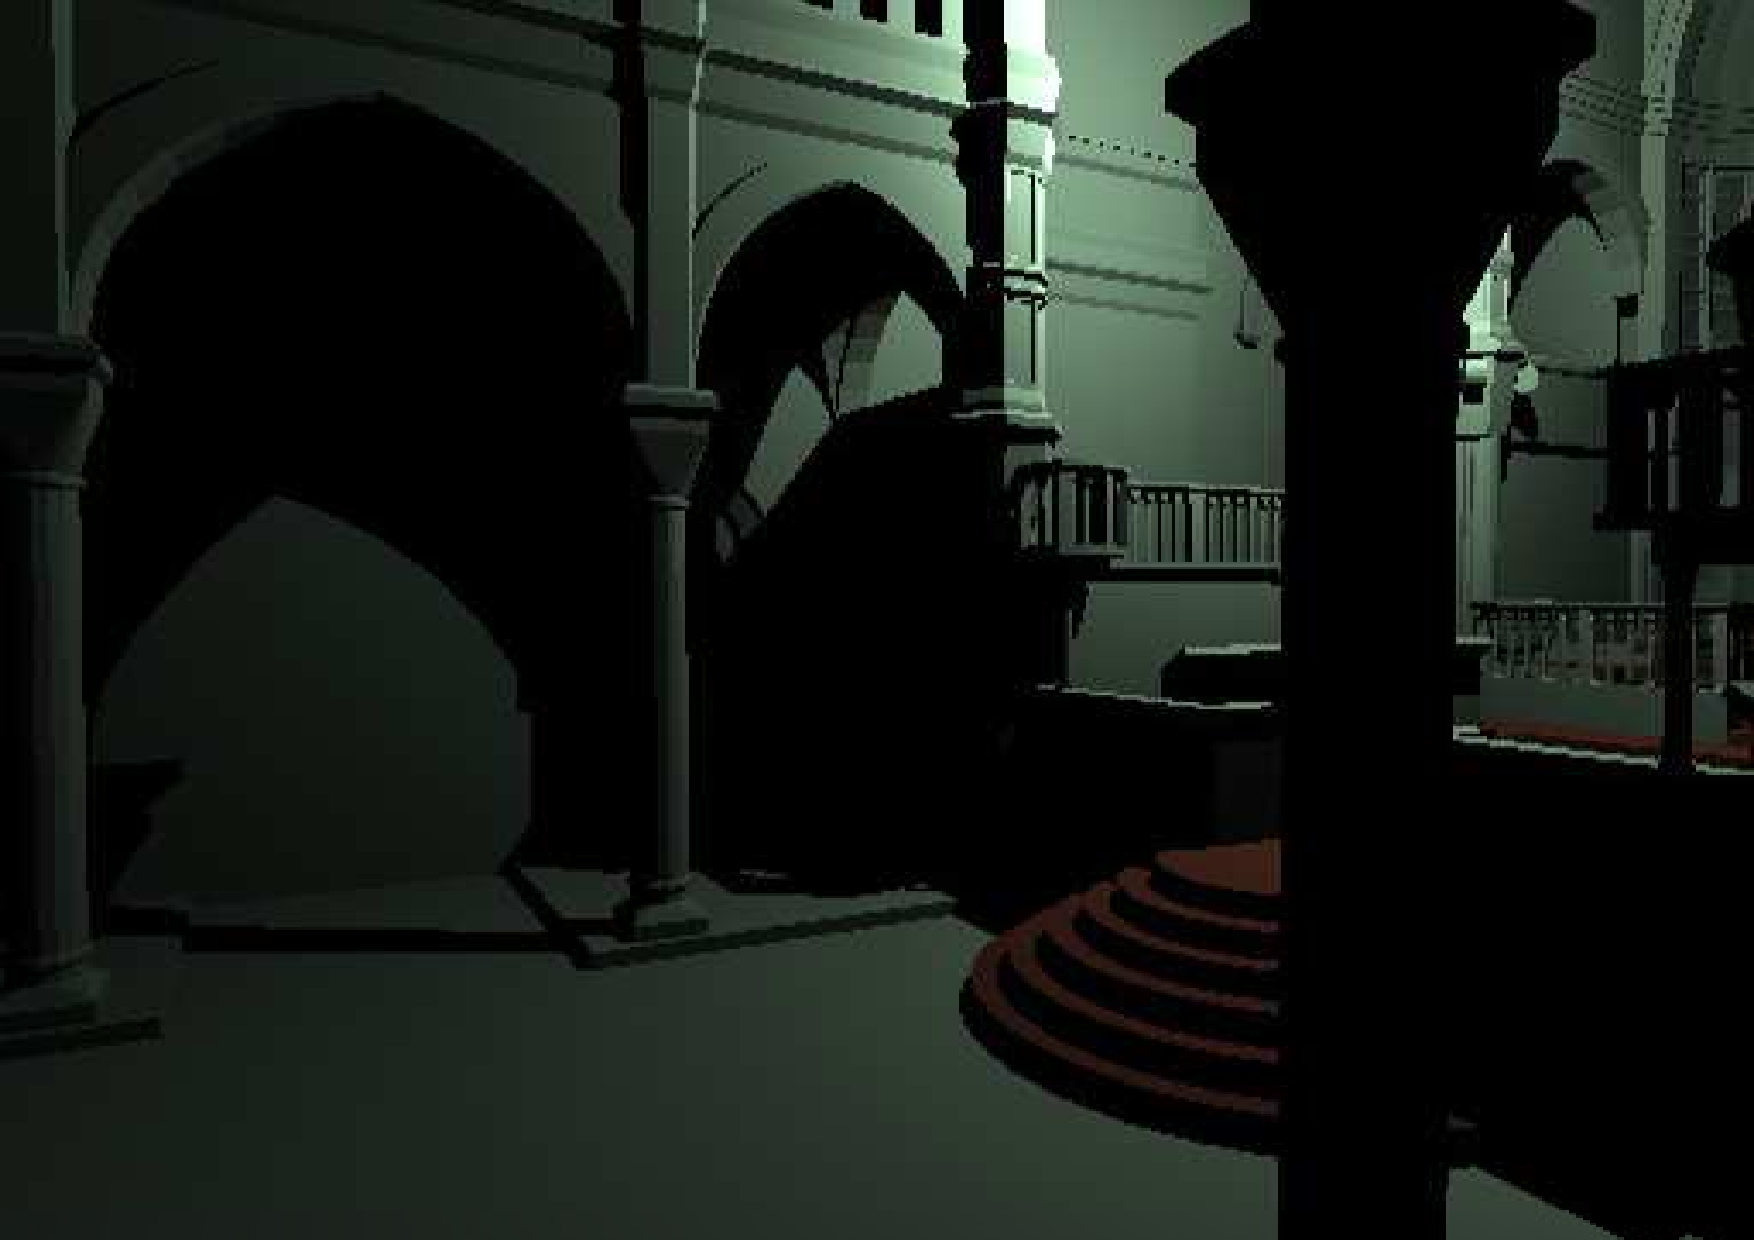
\includegraphics[scale=0.25]{imgs/rt_01.pdf}}
	\subfigure[Test subfigure 2]{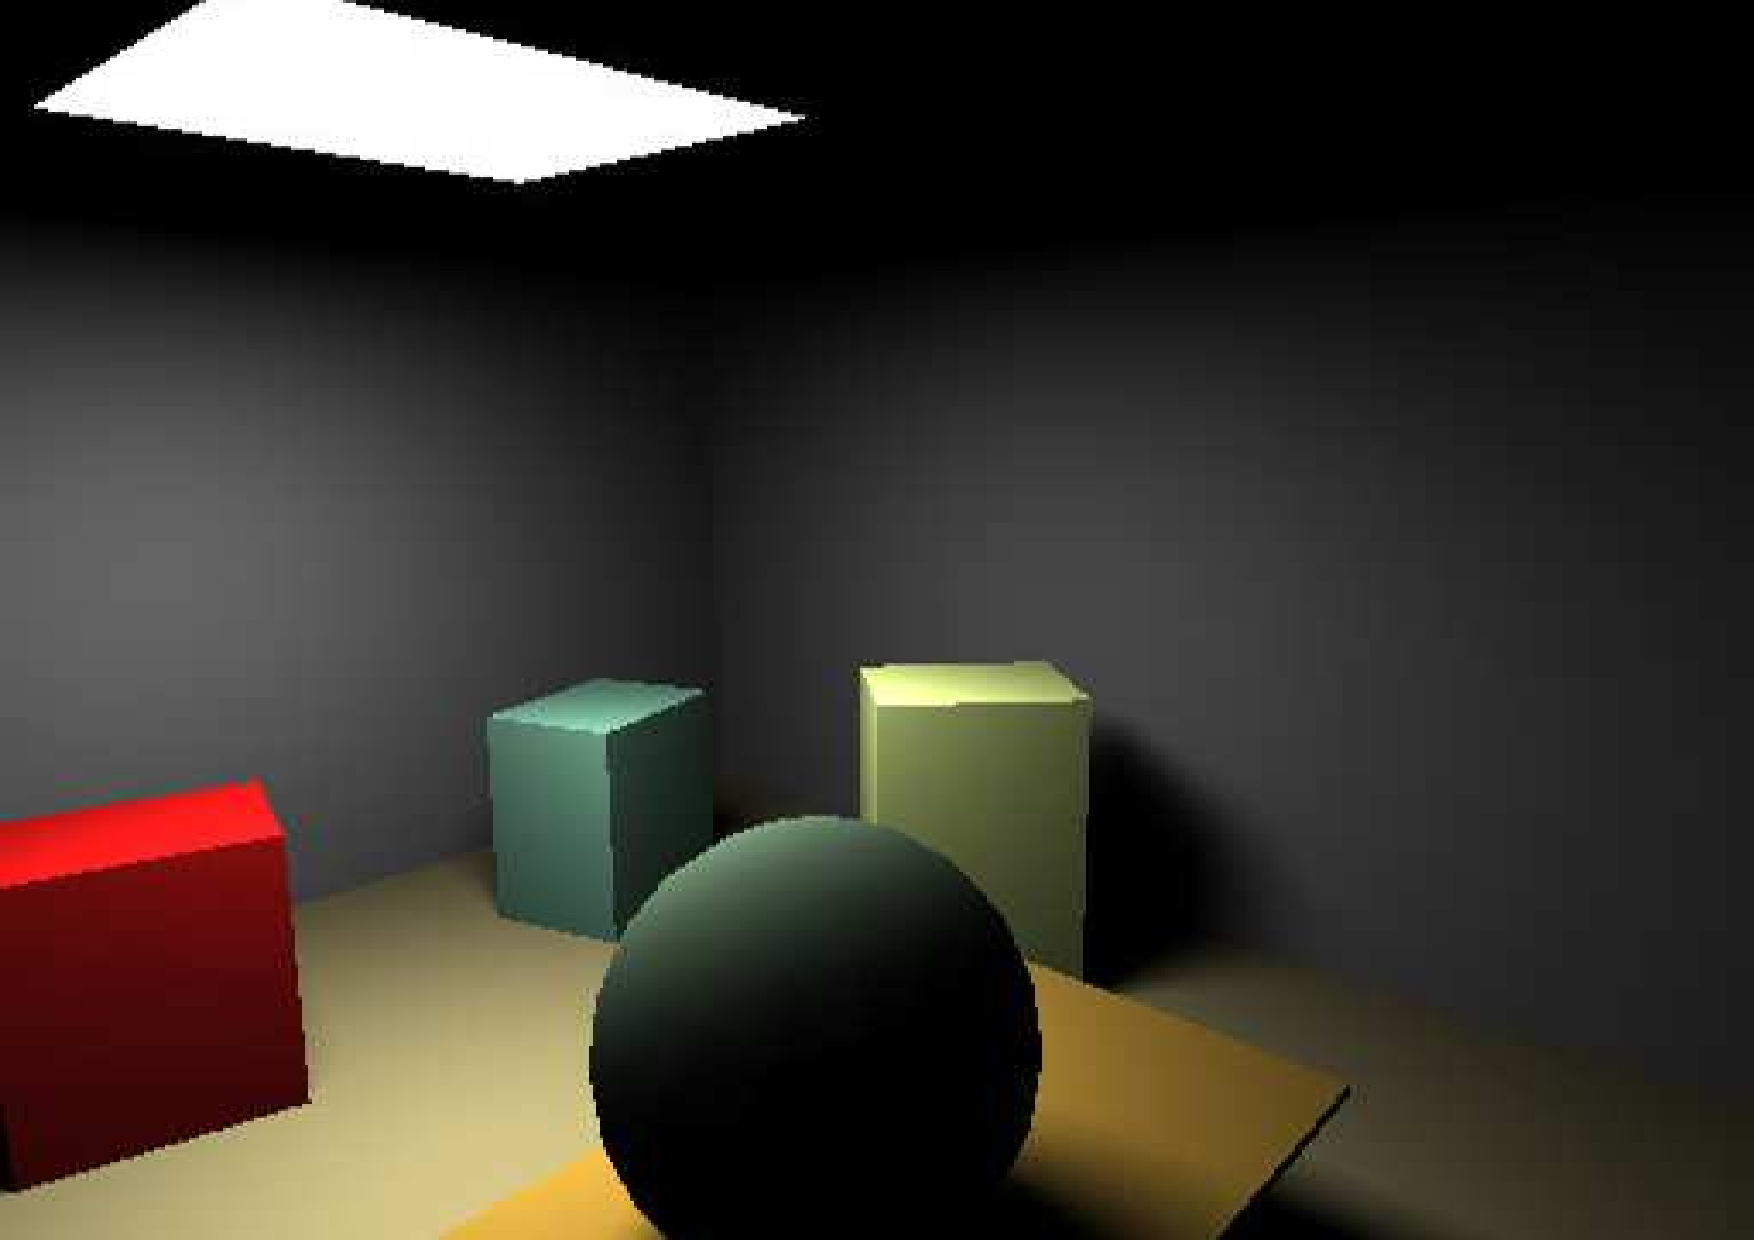
\includegraphics[scale=0.25]{imgs/rt_02.pdf}}
	}
    \renewcommand{\thefigure}{\thechapter.\arabic{figure}}
    \caption[]{The scenes rendered using Monte Carlo ray tracing by our test program. }
    \label{fig:rt_images} 
\end{center} 
\end{figure}

The classic ray tracing technique became popular in Computer Graphics since 1980 with an introduction of the recursive ray-tracing algorithm by Whitted \cite{Whitted1980}. It is an elegent and simple algorithm for easily rendering shadows and specular surfaces. 

The ray tracing algorithm can be broke down into two stages: intersection query and shading. In the first stage, as shown in figure \ref{fig:ray_tracing}, for each pixel on our viewing plane, one of more rays (if the multi-sampling is enabled for better image quality) are shot into the scene, these rays directly from the observer are \emph{primary rays}. Then we are trying to find intersection points with the closest object to observer. In the shading stage, at each intersection point the direct illumination is computed based on the BRDF determined by the surface material, the computed radiance is converted to the color of the corresponding pixel. The visibility of the light sources can be evaluated with shadow rays. If the surface material is specular then a specular ray is traced in the reflected or transmitted direction. The indirect illumination can be computed by spawning and tracing reflected or refracted rays (called \emph{secondary rays}) from the intersection points and repeate the ray tracing recursively. 

\begin{figure}[htp] 
    \centering 
    \fbox{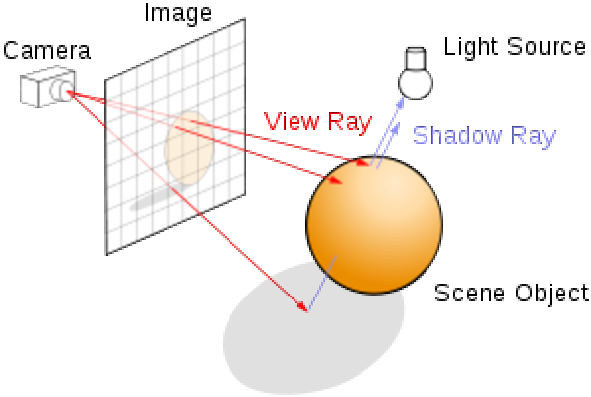
\includegraphics{imgs/ray_tracing.pdf}}
    \renewcommand{\thefigure}{\thechapter.\arabic{figure}}
    \caption[]{Ray Tracing.}
    \label{fig:ray_tracing} 
\end{figure} 

Ray tracing is not a full global illumination algorithm since it cannot handle the computation of the indirect illumination on diffuse surfaces, it can only compute the illumination for perfect specular material by tracing a ray in the refracted or mirror direction. To simulate the phenomena such as soft shadows, it is necessary to employ Monte Carlo sampling techniques\cite{Kajiya:1986:RE:15922.15902}. 

The idea of Monte Carlo technique is to generate a large amount of samples of the rays and evaluate the LTE for every sample using the classic ray tracing technique and average all the results with the Monte Carlo integration to converge the final solution. 

Monte Carlo integration is a method for using random sampling to estimate the values of integrals. In order to estimate the value of integtral \( \int f(x)dx \) one needs only to be able to evalueate the integrand at arbitrary points in the domain. 

The Monte Carlo estimator approximates the value of an arbitrary integral. Suppose \( \int_{a}^{b}f(x)dx \) is an one-dimensional integral we want to evaluate, given a suply of uniform random variables \( X_{i} \in [a, b] \), we can define the Monte Carlo estimator: 
\begin{equation}
F_{N} = \frac{b-a}{N}\sum_{\substack{0<i<N}}f(X_{i})
\end{equation}

and the expected value of \(F_{N}\), \(E[F_{N}]\), is in fact equal to the integral. This fact taks just a few steps to be demonstrated (see p. 541-542 in \cite{Pharr:2010:PBR:1854996}). 

Monte Carlo ray tracing has several advantage over classic ray tracing: 

\begin{itemize} 

\item All global illumination effects can be simulated.

\item Low memory consumption. 

\item Result is correct exception for variance (visible as noise). 

\end{itemize} 

The main disadvantage of Monte Carlo method is that it requires huge amount of samples to minimize the errors. In order to reduce the errors in half, it requires evaluation of four times as many samples. Fortunately many techniques we can use to reduce the numbers of samples to compute while maintain an acceptable image quality. A commonly employed method is importance smapling. Instead of generate samples rays blindly, we only send rays where the LTE's integrand has high values. This is easy for direct lighting but difficult for indirect lighting as the it is impossible to know where the largest illumination contribution comes from. Combining the other compoents like the BRDF \(f_{r}\) and incident lighting \(L_{i}\) into one importance sampling approach is more challenging for global illumination. Solutions to this issue includes multiple-importance sampling technique and bi-directional path tracing\cite{Lafortune93bi-directionalpath}.

Accelerating ray tracing by exploiting the hardware have been an active research field as well. Optimizations for modern multi-cores CPUs for ray tracing renderer are presented\cite{Wald:2002:IGI:581896.581899}. 

\subsection{Photon Mapping}


\subsubsection{Concept} 

Photon mapping was developed by Jensen \cite{HenrikWannJensen2004} as an efficient alternative to the Monte Carlo ray tracing tecnniques especially for simulating the focused light effects, such as caustics. Photon mapping is a two-pass algorithm, photon tracing and radiance estimation. 

\paragraph{Photon Tracing} 
Photon tracing is the process of shooting photons from the light sources and tracing them into the scene similar to stardard ray tracing, a global data structure constructed to store the photons is called photon map. When a photon hits a diffuse surface, its position, incident direction and power will be stored in the photon map. Jenson suggests that using balanced kd-tree data structure to organize the photons data, since the kd-tree is beneficial to the next pass, radiance estimate. Whether the photon is absorbed or reflected is determined by the surface's BRDF. Photons that hits the specular surface will not be stored because the probability of have a incoming photons from specular direction is zero. Instead, these surfaces are rendered using standard ray tracing. 

\paragraph{Radiance Estimate}
Given the photon map, we can perform density estimate on certain surface point to calculate reflected radiance. The direct illumination and specular surfaces can be rendered using Monte Carlo ray tracing. As shown in figure \ref{fig:photon_density_estimate}, we collecting \(n\) photons samples within the a sphere make the estimate of the reflected radiance at any surface location \(x\), as shown in equation \ref{eq:photon_estimate}. 

\begin{equation}
L_r(x, \omega_{o}) \approx \frac{1}{\pi r^{2}}\sum_{\substack{0<p<N}}f_{r}(x, \omega_{p, o}, \omega_{i})\Delta \Phi_{p}(x,\omega_{p, o}) 
\label{eq:photon_estimate}
\end{equation} 

\begin{figure}[ftp] 
    \centering 
    \fbox{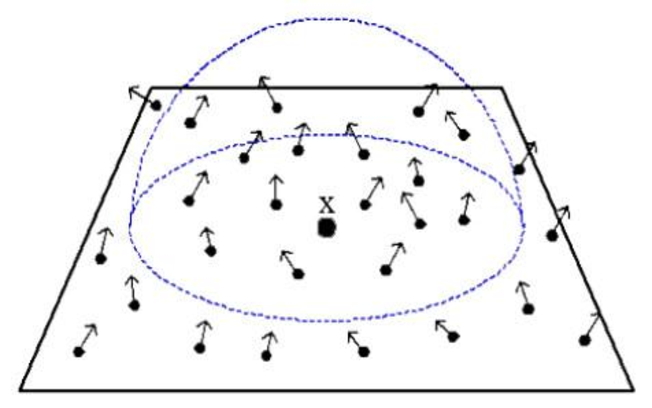
\includegraphics{imgs/photon_density_estimate.pdf}}
    \renewcommand{\thefigure}{\thechapter.\arabic{figure}}
    \caption[]{Photon density estimate.}
    \label{fig:photon_density_estimate} 
\end{figure} 


%%%%%%%%%%%%%%%%%%%%%%%%%%%%%%%%%%%%%%%%%%%%%%%%%%%%%%%%%%%%%%%%%%%%%%%%%%

\section{Photon Mapping On GPU} 

\subsection{KD-Tree Construction} \label{subsec:kdtree_construction} 

\subsection{K Nearest Neighbor Search Using GPU}






